\subsection{LQG-Regler}
    Die kombination eines LQR-Reglers und eines Luenberer-Observer nennt man \textit{LQG (Linear Quadratic Gaussian)}. Anstatt den realen Zustand $x(t)$ wird nun seine Schätzung $\widehat{x}(t)$ zurückgeführt.
    \begin{equation*}
        u(t) = -K\cdot\widehat{x}(t)
    \end{equation*}
    \begin{figure}[H]
        \centering
        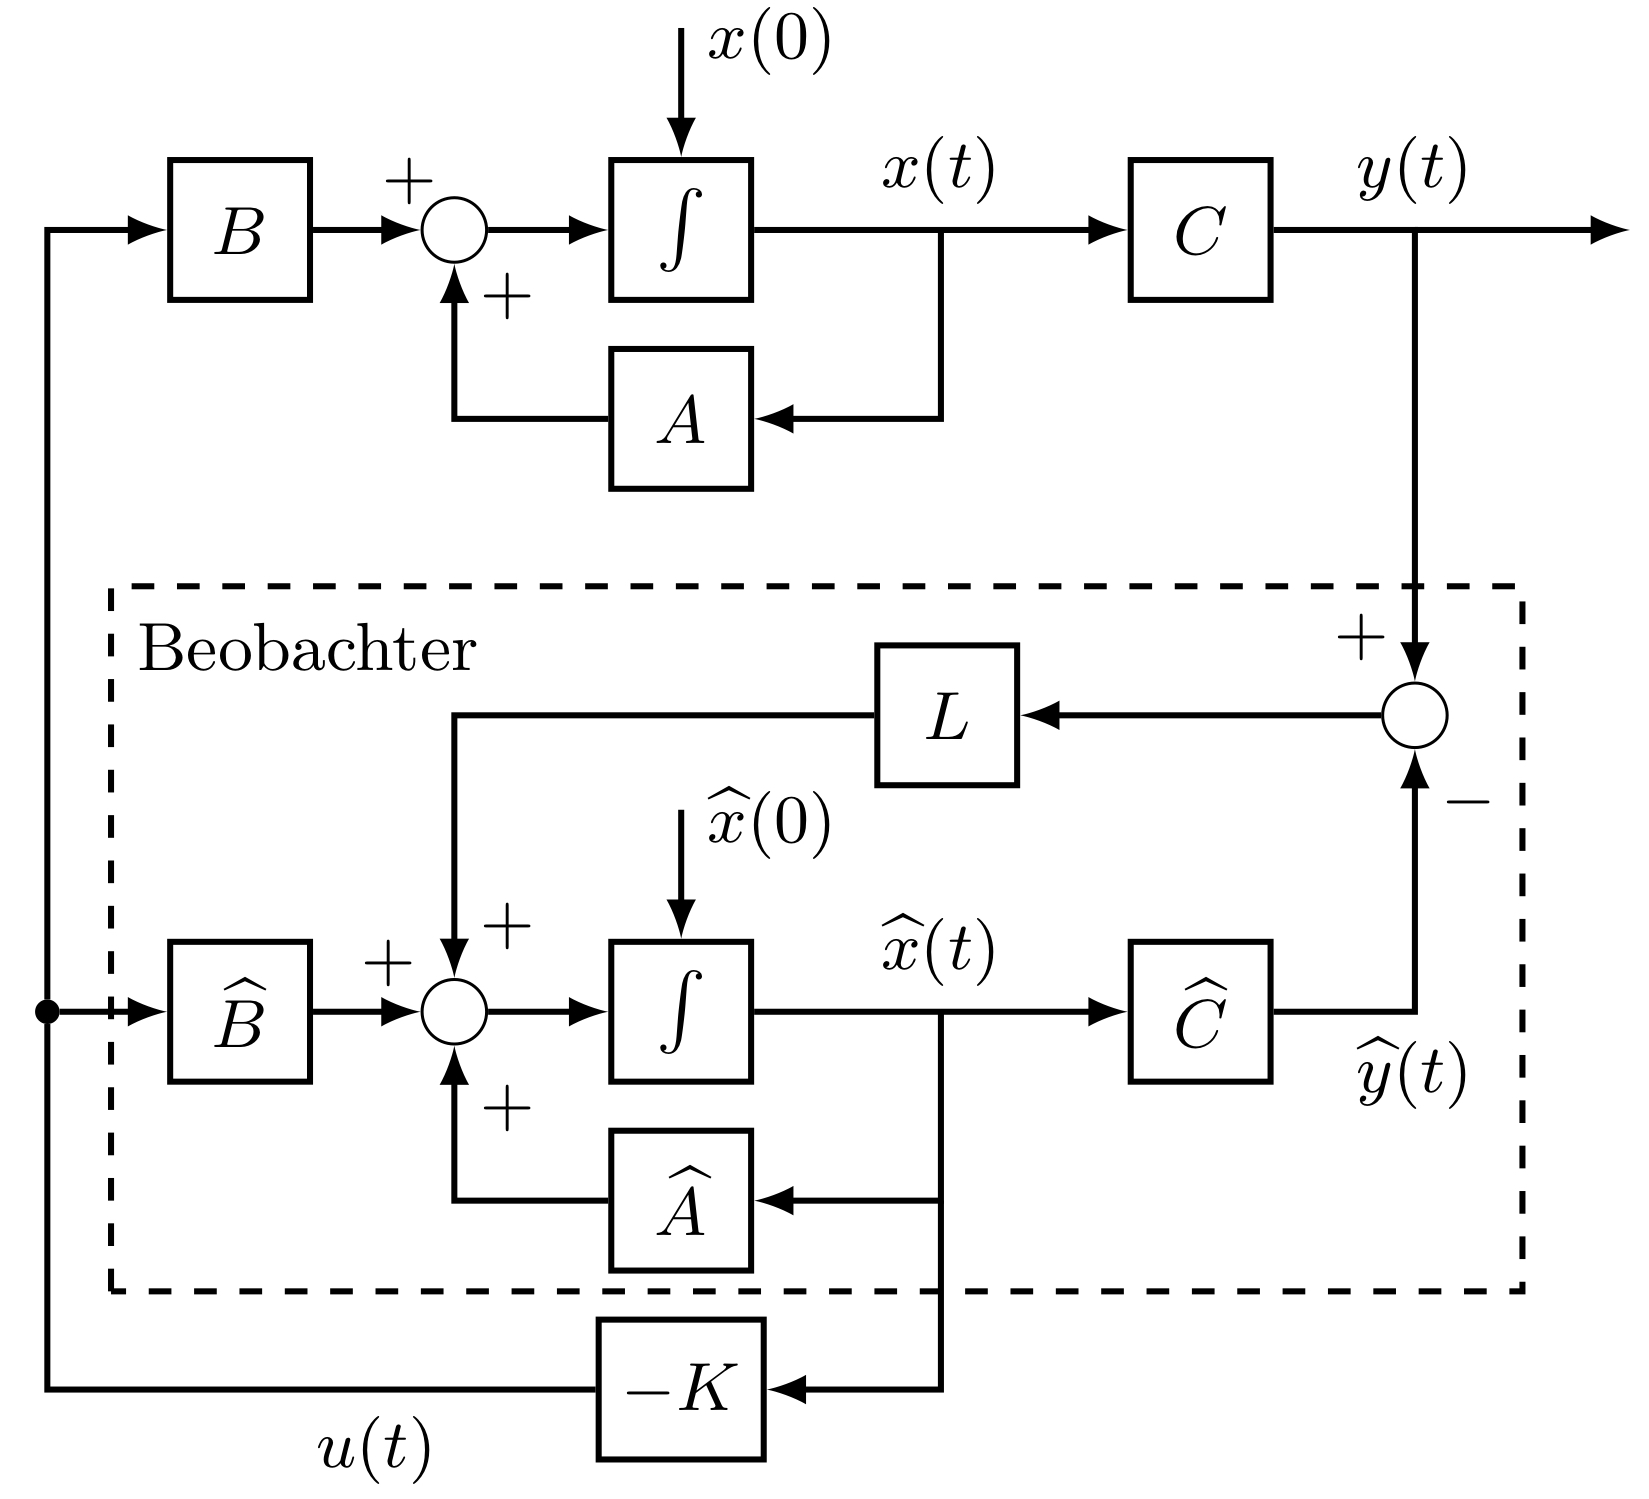
\includegraphics[width = 0.6\linewidth]{images/10/LQG_vanilla.jpeg}
        \caption{Blockdiagramm eines LQG-Reglers}
    \end{figure}
    
    \begin{figure}[H]
        \centering
        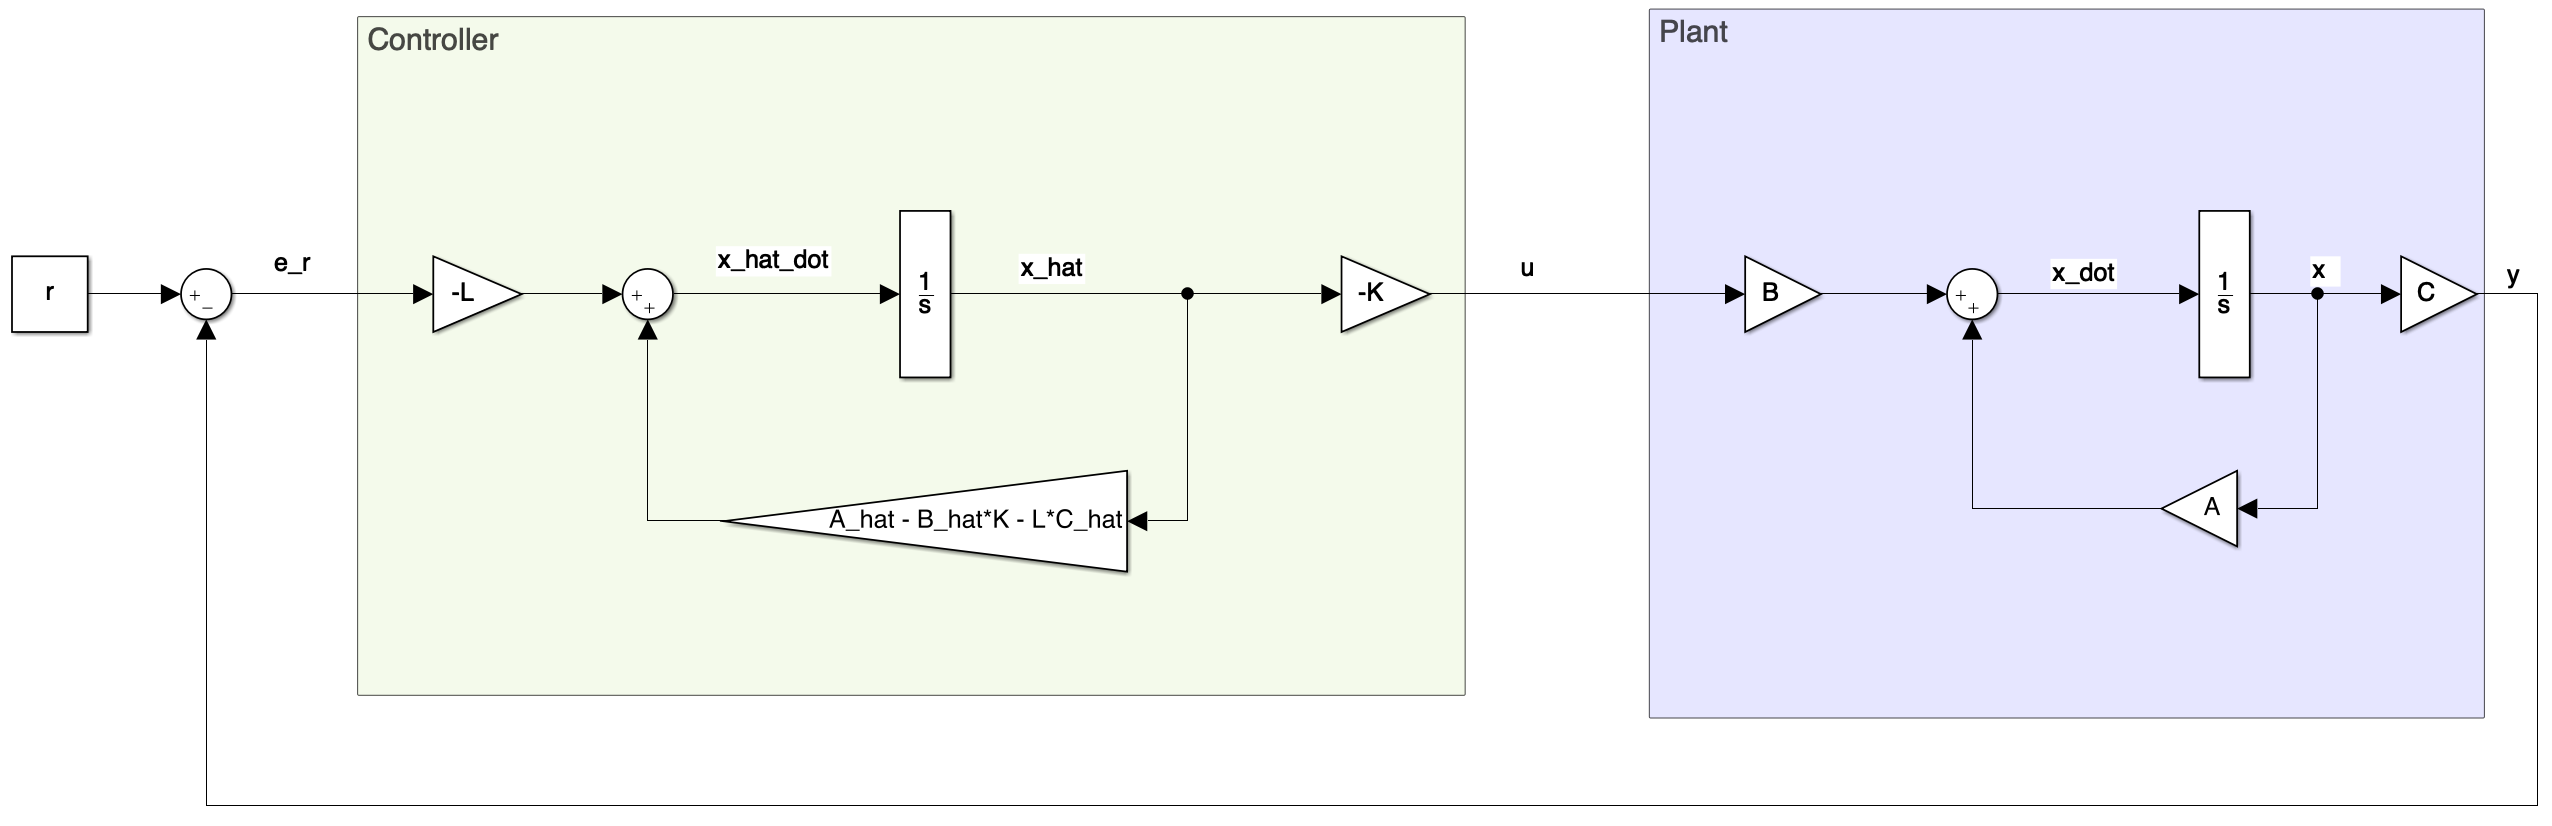
\includegraphics[width = \linewidth]{images/10/LQR_alt.png}
        \caption{Alternative Darstellung des LQR-Reglers}
    \end{figure}
    
\subsection{Stabilität des LQG}
    Unter der Annahme, dass die Matrizen $\{A, B, C\}$ exakt bekannt sind ergibt sich folgende Dynamik
    \begin{equation*}
        \Tilde{x}(t) = \begin{bmatrix}x(t)\\\widehat{x}(t)\end{bmatrix},\quad
        \frac{d}{dt}\Tilde{x}(t) = 
        \underbrace{\begin{bmatrix}
        A   &   -B\cdot K\\
        L\cdot C & A-B\cdot K-L\cdot C
        \end{bmatrix}}_{\Tilde{A}_{\textnormal{cl}}}
        \cdot \Tilde{x}(t)
    \end{equation*}
    Die Stabilität ist durch die Eigenwerte von $\Tilde{A}_{\textnormal{cl}}$ gegeben. Sind aber in dieser Form nicht einfach zu berechnen.
    
    \subsubsection{Separation Principle}
        Verwendet man die Koordinatentransformation
        \begin{equation*}
            \Tilde{z} = 
            \begin{bmatrix}
            x(t)\\e(t)
            \end{bmatrix}
            =
            \begin{bmatrix}
            x(t)\\x(t)-\widehat{x}(t)
            \end{bmatrix}
            =
            \begin{bmatrix}
            I_{n\times n} & 0\\I_{n\times n} & I_{n\times n}
            \end{bmatrix}
            = \underbrace{T^{-1}}_{=T}\cdot\widehat{x}(t)
        \end{equation*}
        Daraus ergib sich folgende Dynamik
        \begin{equation*} 
            \frac{d}{dt}\Tilde{z}(t) = 
            \underbrace{\begin{bmatrix}
            A-B\cdot K   &   B\cdot K\\
            0 & A-L\cdot C
            \end{bmatrix}}_{\textnormal{gleiche EW wie }\Tilde{A}_{\textnormal{cl}}}
            \cdot\Tilde{z}(t) = T^{-1}\cdot\Tilde{A}_\textnormal{cl}\cdot T\cdot\Tilde{z}(t)
        \end{equation*}
        Daraus folgt direkt
        \begin{align*}
            \operatorname{eig}(T^{-1}\cdot\Tilde{A}_\textnormal{cl}\cdot T) &= \operatorname{eig}(\Tilde{A}_\textnormal{cl}) = \operatorname{eig}(A-B\cdot K)\cup \operatorname{eig}(A-L\cdot C)\\ 
            &\therefore \Tilde{A}_\textnormal{cl}\,\textnormal{ist Hurwitz}
        \end{align*}